\section{Aplicación final}
\label{sec:aplicacionFinal}
Una vez los modelos estaban preparados era necesaria una aplicación a modo de demostración que se pueda ejecutar en las gafas de \gls{vr} y con el traje de caputra de movimiento.
La aplicación consta de un panel en el que introduces la IP de la máquina que tiene el servidor de Tensor ejecutándose con el modelo y la aplicación de Axis Studio para poder utilizar el traje.
Además, tiene un panel de texto en el que aparecen los resultados de la predicción y un NPC que reacciona a tus gestos. En la figura \ref{fig:DemoCaptura} se puede ver una captura de esa aplicación.

\begin{figure}[H]
    \centering
    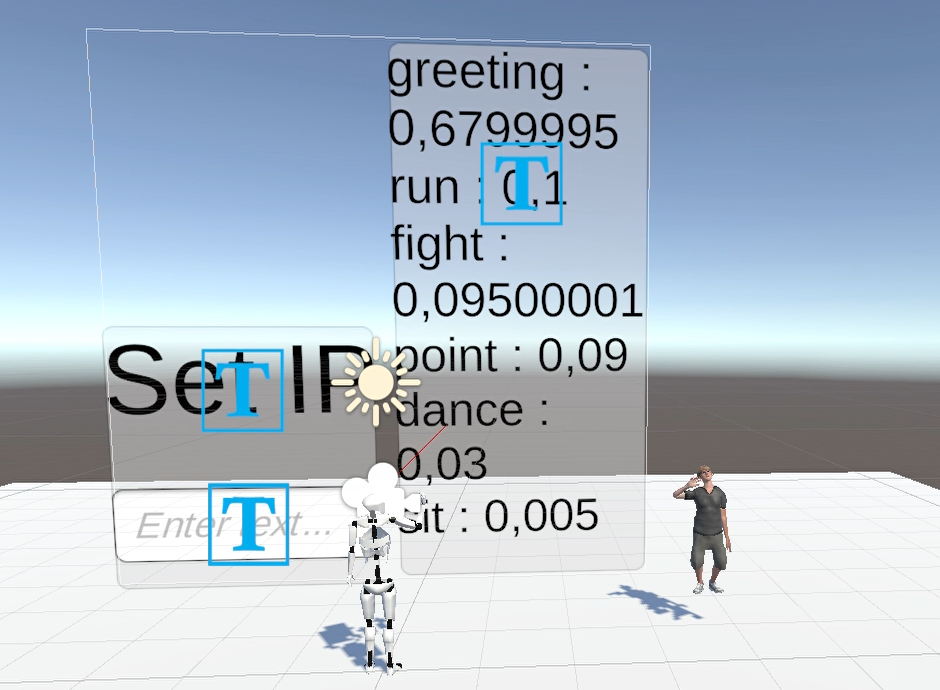
\includegraphics[width=0.5\textwidth]{Imagenes/Bitmap/Demo.PNG}
    \caption{Captura de la aplicación final desde el editor de Unity}
    \label{fig:DemoCaptura}
\end{figure}

\subsection{Funcionamiento de la aplicación}
Al introducir la IP en el cuadro de texto la aplicación se conecta con el traje y el servidor de Tensor.
La conexión con el traje es la misma que la del apartado \ref{subsec:NeuronMocapLive}, mientras que para el servidor se utiliza una \gls{API REST} mediante UnityWebRequest,\footnote{Página de la documentación de Unity: \url{https://docs.unity3d.com/ScriptReference/Networking.UnityWebRequest.html}} una API de Unity para comunicarse con servidores web.
Esta ejecución se hace mediante una corrutina, la cual al principio espera la cantidad de tiempo óptima entre frame y frame que se determinó en el entrenamiento del modelo usado (en nuetro caso el Random Forest con 0.8 segundos).

La información de los huesos se guarda en una cola, donde se guarda la información actual y, una vez enviado al servidor, se elimina la más antigua, siendo siempre el tamaño de la cola de máximo dos elementos.
Al pasar estos segundos la aplicación manda al servidor la información de los huesos en el frame actual y en el frame de hace 0.8 segundos (previamente guardado) en formato JSON mediante POST con protocolo HTTP, a lo que el servidor le responde con dos listas en formato JSON: una con los gestos y otra con el score que ha conseguido cada gesto en la predicción, coincidiendo el índice del score de un gesto con el índice del gesto de la anterior lista.
Para hacer todas las conversiones entre cadenas de texto y el formato JSON se ha usado la clase JsonUtilty nativa en Unity.

Una vez se tenga la respuesta del servidor empieza de nuevo la corrutina, se ordena de mayor a menor score las predicciones mediante bubble sort para escribirlas en el panel correspondiente y se ejecuta la animación de respuesta del \gls{npc}.
Las animaciones de respuesta que tiene a los gestos se puede ver en la tabla \ref{tab:gestos-reaccion}

\begin{table}[H]
    \begin{center}
        \begin{tabular}{| c | c |}
            \hline
            Gesto    & Animación de reacción \\ \hline
            Bailar   & Aplaudir              \\
            Saludar  & Saludar               \\
            Señalar  & Mirar                 \\
            Sentarse & Sentarse              \\
            Pelear   & Pose defensiva        \\
            Correr   & Correr                \\ \hline
        \end{tabular}
        \caption{Reacción del \gls{npc} al gesto predicho del jugador}
        \label{tab:gestos-reaccion}
    \end{center}
\end{table}

Si hay un error de conexión en mitad de la ejecución se deberá ingresar de nuevo la IP de la máquina host en el campo de texto para reintentarlo.

En la figura \ref{fig:Demo} se puede ver el diagrama de flujo de esta aplicación.

\newpage
\begin{figure}[H]
    \centering
    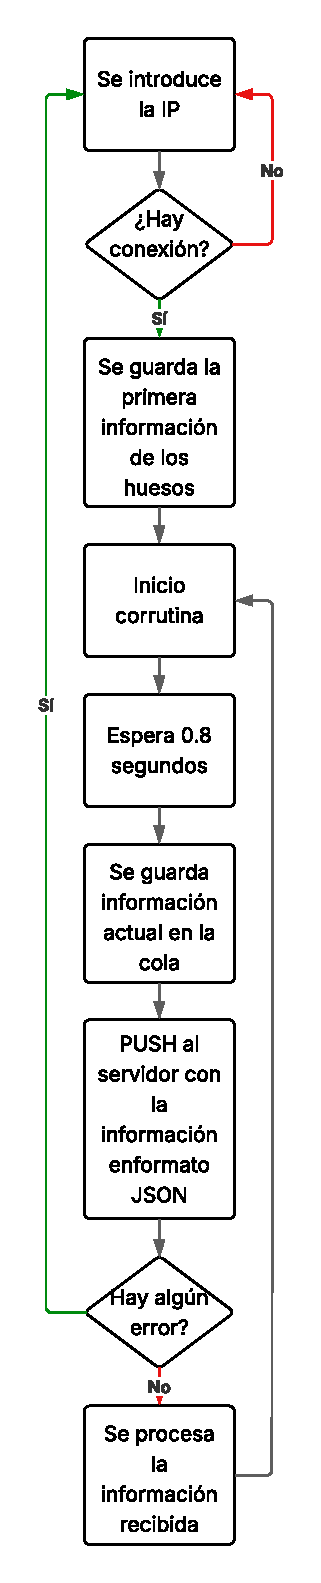
\includegraphics[width=0.3\textwidth]{Imagenes/Vectorial/FlujoAppFinal.pdf}
    \caption{Diagrama de flujo de la aplicación de demostración}
    \label{fig:Demo}
\end{figure}